\documentclass[a4paper, 12pt]{article}

% osnovni paketi za jezik in kodiranje znakov
\usepackage[slovene]{babel} 
\usepackage[utf8]{inputenc}
\usepackage[T1]{fontenc}
\usepackage{lmodern}

% dodatni paketi
\usepackage{amsmath, amssymb, amsthm}
% \usepackage[font=small, center]{caption}
\usepackage[hidelinks]{hyperref}
\usepackage{graphicx}
\usepackage{wrapfig}
\usepackage{float}     
\usepackage{geometry}
\usepackage[table]{xcolor} % http://ctan.org/pkg/xcolor
\usepackage{biblatex}
\addbibresource{literatura.bib}


\begin{document}

\begin{titlepage}
    \begin{center}
        \large
        Fakulteta za matematiko in fiziko\\
        Oddelek za matematiko \\
        \vspace{6cm}
        \Huge
        \textbf{Vizualizacija Kakeya-množice} \\
        \vspace{6cm}
        \large
        Terezija Krečič\\
        Pedagoška matematika, 5. letnik\\
        \vspace{1cm}
        Predmet: Matematika z računalnikom \\
        Mentor: Sergio Cabello\\
        \vspace{2cm}
        Ljubljana, 21. 5. 2024
    \end{center}
\end{titlepage}

\newpage


%%%%%%%%%%%%%%%%%%%%%%%%%%%%%%%%%%%%%%%%%%%%%%%%%%%%%%%%%%%%%%%%%

\section*{Uvod}

V tej projektni nalogi je bil cilj vizualizirati Kakeya-množico s pomočjo programa \href{https://ipe.otfried.org/}{Ipe}. Najprej sem morala sploh predelati problem, ki ga je zastavil Kakeya več kot 100 let nazaj, poleg tega pa se še spoznati z novo programsko opremo.

V poročilu bom na kratko predstavila glavno vprašanje in eno strategijo, kako ga rešiti. Vse slike, ki so vključene zraven, sem ustvarila sama s pomočjo Geogebre in omenjenega orodja Ipe. Poročilo je povzeto po Besicovitchevem članku~\cite{Besicovitch}.

%%%%%%%%%%%%%%%%%%%%%%%%%%%%%%%%%%%%%%%%%%%%%%%%%%%%%%%%%%%%%%%%%

\section*{Kakeyev problem igle}

Japonski matematik Sōichi Kakeya je leta 1917 zastavil naslednje vprašanje, ki se ga je v kasnejšem času prijelo ime ``\emph{the Kakeya needle problem}\footnote{Kakeyev problem igle, op. prev.}'':

\vspace{0.2cm}
\begin{center}
    \textbf{Kolikšna je lahko najmanjša ploščina območja, znotraj katerega se daljica dolžine 1 zvezno obrne za 180 °?}
\end{center}
\vspace{0.2cm}

\noindent Poglejmo si tri primere geometrijskih likov, ki ustrezajo pogoju iz vprašanja:

\begin{enumerate}
    \item krog s premerom 1 $ \rightarrow $ ploščina $ = \frac{\pi}{4} \doteq 0{,}79 $
    \item enakostranični trikotnik z višino 1 $ \rightarrow $ ploščina $ = \frac{1}{\sqrt{3}} \doteq 0{,}58 $
    \item deltoida\footnote{za konstrukcijo deltoide gl.~\cite{deltoida}, za animacijo obračanja igle znotraj nje pa~\cite{kakeya_wiki}}, včrtana v krog s premerom $ \frac{2}{3} $ $ \rightarrow $ ploščina $ = \frac{\pi}{8} \doteq 0{,}39 $
\end{enumerate}

\begin{figure}[h!]
    \centering
    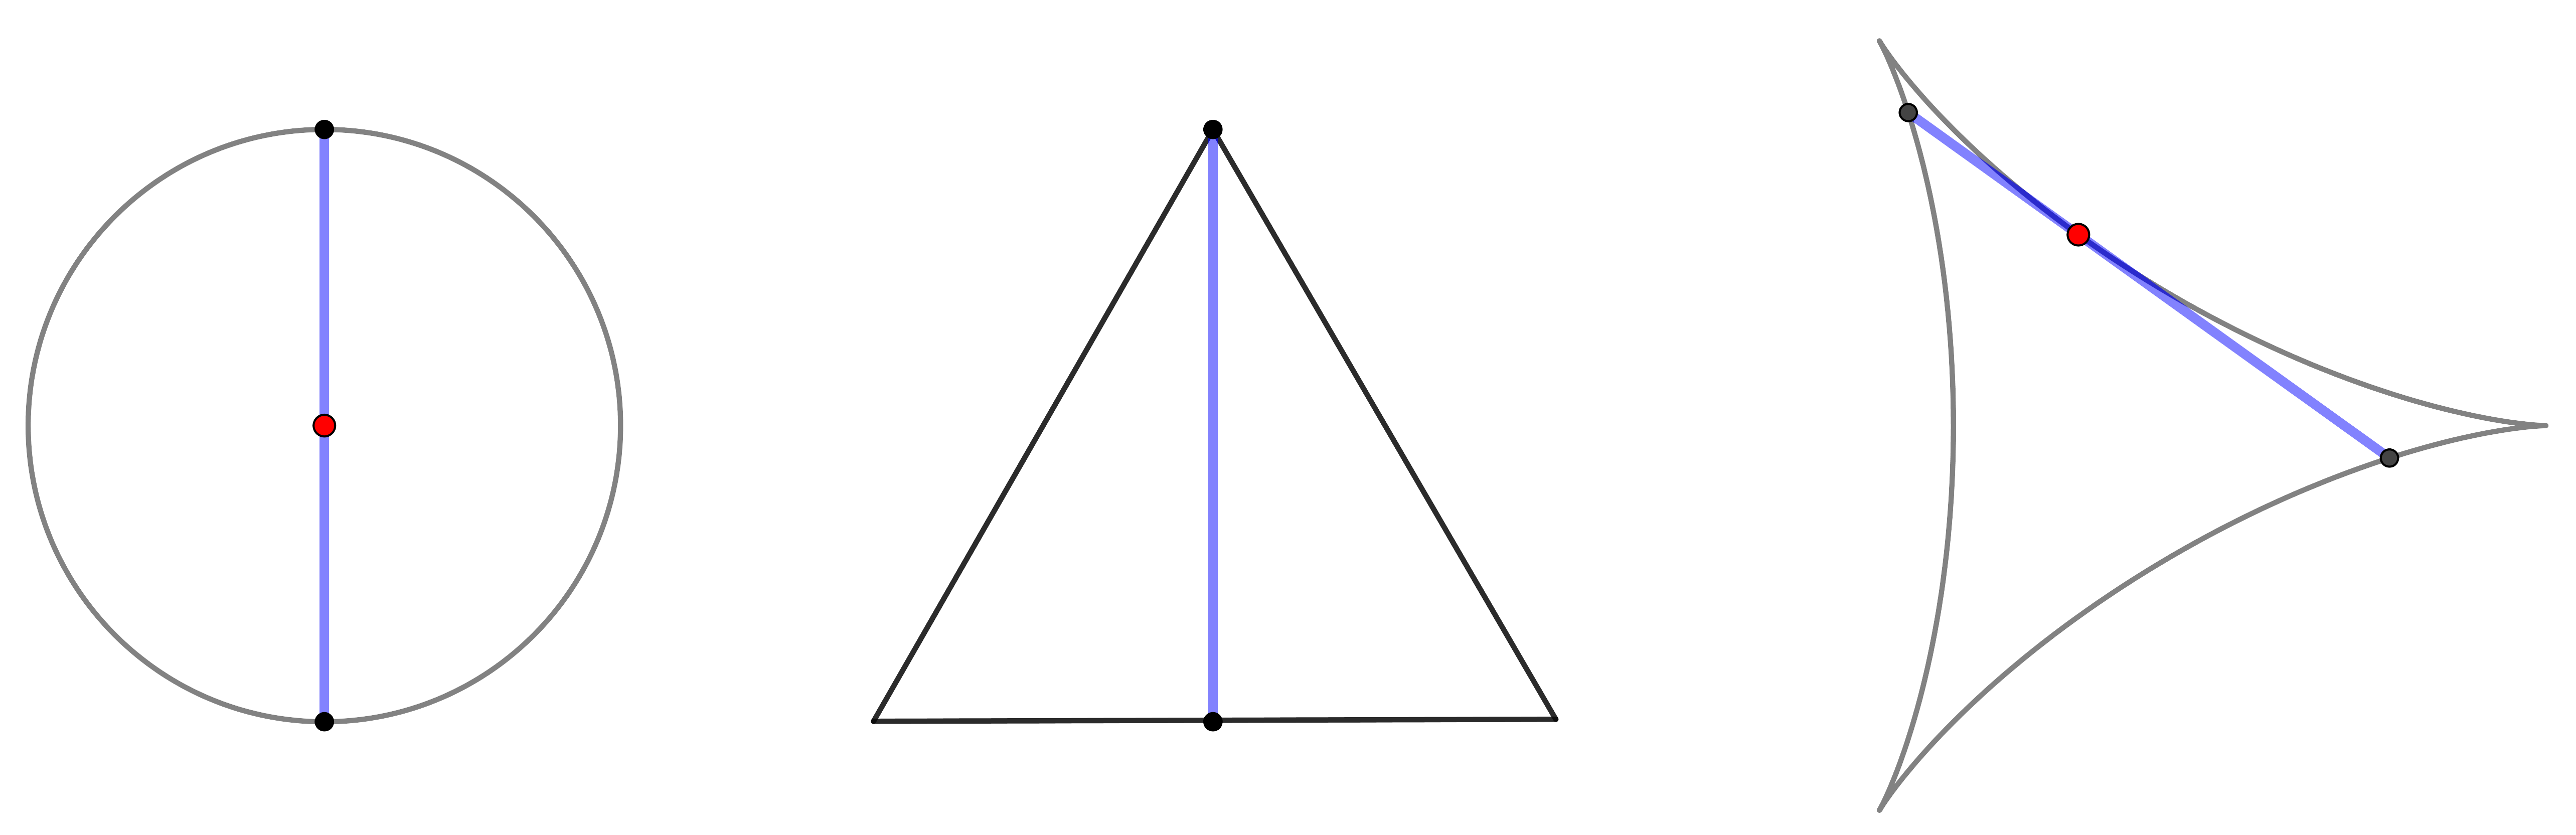
\includegraphics[width=0.9\textwidth]{geogebra_slike/prevelike_ploscine.png}
    \caption{Primeri, ki ustrezajo pogoju.}
    \label{primeri}
\end{figure}

Nekaj časa je veljalo, da je tretji primer, tj. deltoida, odgovor na vprašanje Kakeye, vendar je ruski matematik Abram Besicovitch uspel dokazati, da \textbf{spodnja meja za iskano ploščino \emph{ne} obstaja}. K enostavnejši konstrukciji primera takega lika je pripomogel tudi nemški matematik Oskar Perron, svoj del pa prispeval še madžarsko-danski matematik Gyula Pál.

%%%%%%%%%%%%%%%%%%%%%%%%%%%%%%%%%%%%%%%%%%%%%%%%%%%%%%%%%%%%%%%%%

\section*{Ideja za konstrukcijo}

Vzemimo enakokraki pravokotni trikotnik s katetama dolžine 2. Če v središče hipotenuze postavimo en konec enotske daljice, lahko njen drugi konec opiše kot 180 °, ne da bi kakršenkoli del daljice zapustil trikotnik.

\begin{figure}[h!]
    \centering
    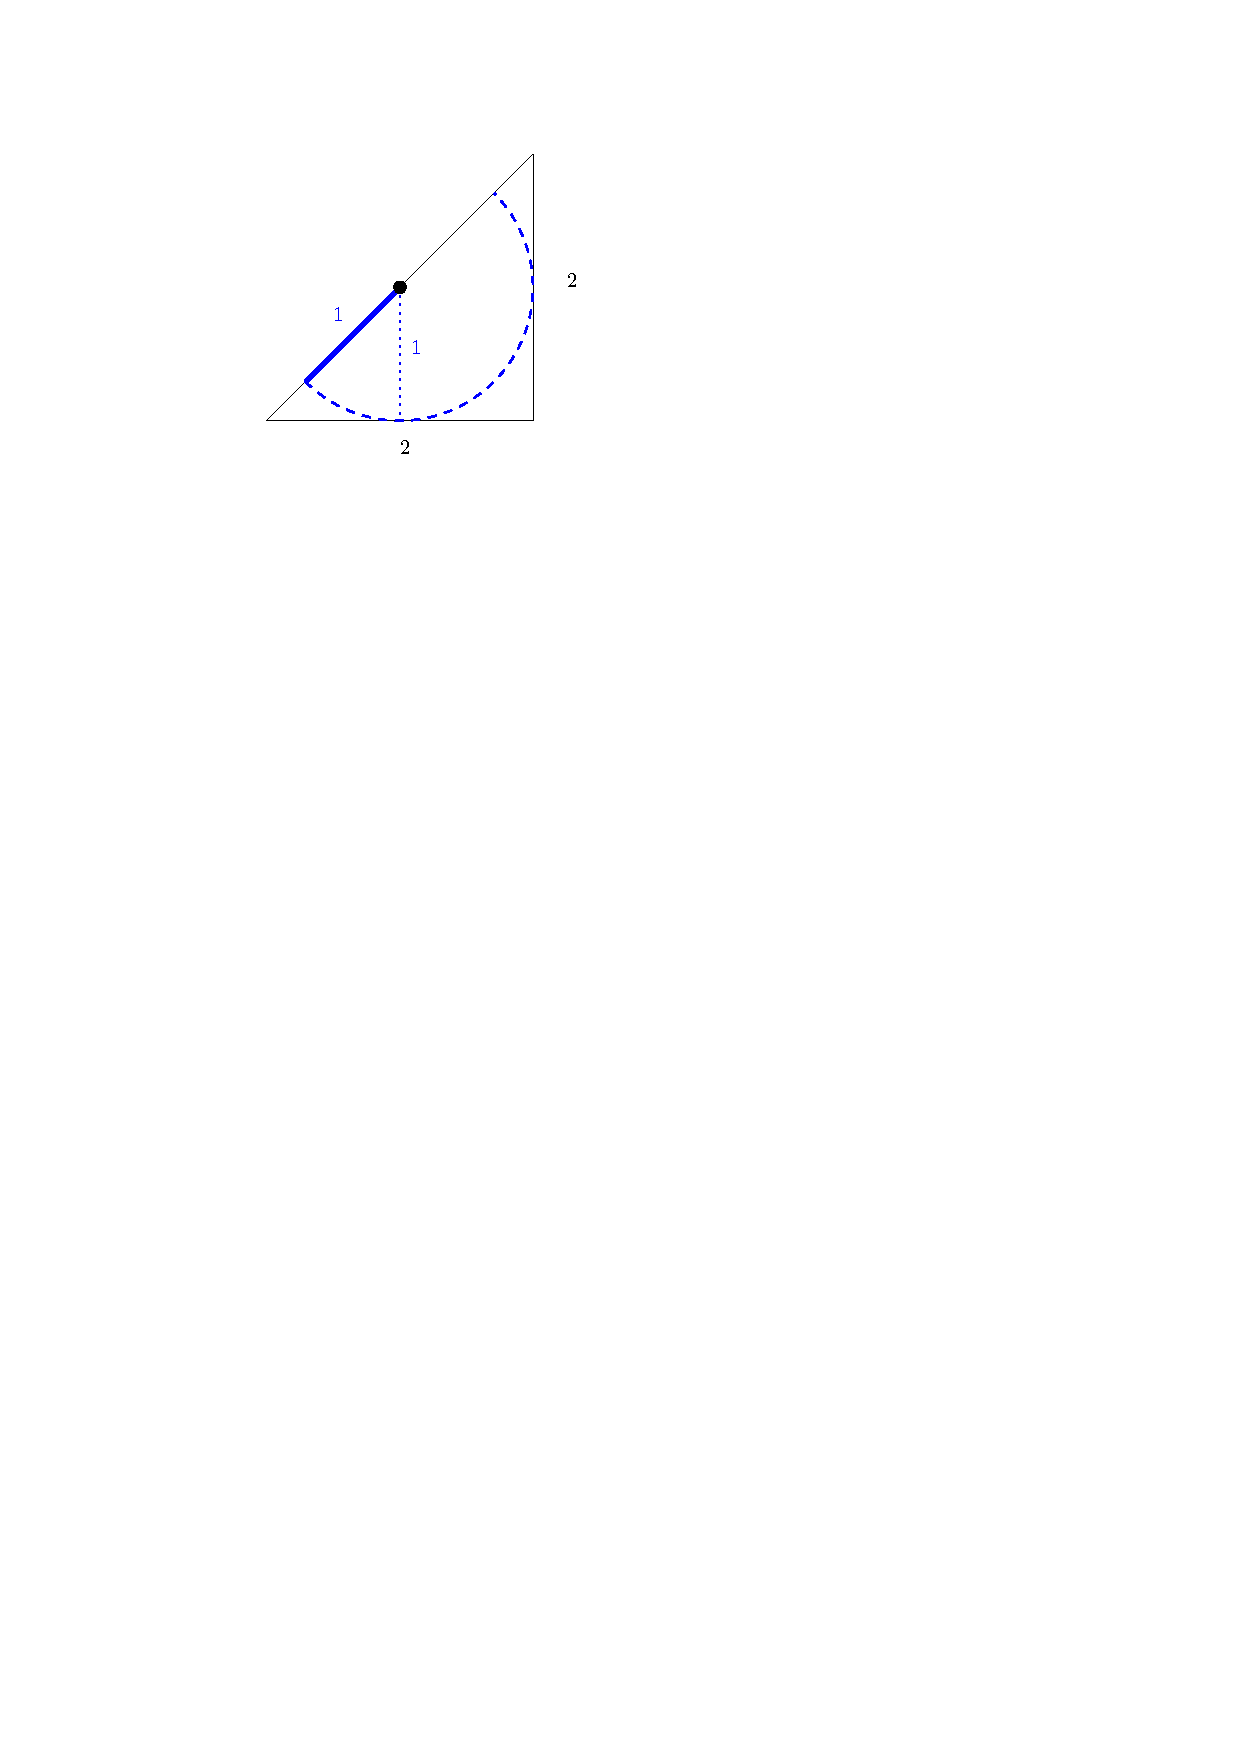
\includegraphics[width=0.3\textwidth]{ipe_slike/trikotnik.pdf}
    % \caption{Primeri, ki ustrezajo pogoju.}
    \label{trikotnik}
\end{figure}



%%%%%%%%%%%%%%%%%%%%%%%%%%%%%%%%%%%%%%%%%%%%%%%%%%%%%%%%%%%%%%%%%


%%%%%%%%%%%%%%%%%%%%%%%%%%%%%%%%%%%%%%%%%%%%%%%%%%%%%%%%%%%%%%%%%


%%%%%%%%%%%%%%%%%%%%%%%%%%%%%%%%%%%%%%%%%%%%%%%%%%%%%%%%%%%%%%%%%


%%%%%%%%%%%%%%%%%%%%%%%%%%%%%%%%%%%%%%%%%%%%%%%%%%%%%%%%%%%%%%%%%

%%%%%%%%%%%%%%%%%%%%%%%%%%%%%%%%%%%%%%%%%%%%%%%%%%%%%%%%%%%%%%%%%

\section*{Zaključek}

%%%%%%%%%%%%%%%%%%%%%%%%%%%%%%%%%%%%%%%%%%%%%%%%%%%%%%%%%%%%%%%%%

% \nocite{*}      % navede tudi vire, ki jih ne citiras
\printbibliography[heading=bibintoc, title={Literatura}]

%%%%%%%%%%%%%%%%%%%%%%%%%%%%%%%%%%%%%%%%%%%%%%%%%%%%%%%%%%%%%%%%%

\end{document}